\documentclass[aspectratio=169, 11pt]{beamer}

% ─── Theme and colors ─────────────────────────────────────────────────────────
\usetheme{Madrid}
\usecolortheme{seahorse}
\definecolor{hadoopYellow}{RGB}{255, 205, 0}
\definecolor{hadoopDark}{RGB}{30, 41, 59}
\definecolor{hadoopBlue}{RGB}{59, 130, 246}
\definecolor{hadoopGreen}{RGB}{34, 197, 94}
\definecolor{hadoopRed}{RGB}{239, 68, 68}
\definecolor{codeBg}{RGB}{241, 245, 249}

\setbeamercolor{palette primary}{bg=hadoopDark, fg=white}
\setbeamercolor{palette secondary}{bg=hadoopBlue, fg=white}
\setbeamercolor{palette tertiary}{bg=hadoopBlue, fg=white}
\setbeamercolor{title}{fg=hadoopDark}
\setbeamercolor{frametitle}{fg=hadoopDark, bg=white}
\setbeamercolor{block title}{bg=hadoopBlue, fg=white}
\setbeamercolor{block body}{bg=codeBg}
\setbeamercolor{block title alerted}{bg=hadoopRed, fg=white}
\setbeamercolor{block title example}{bg=hadoopGreen, fg=white}

\setbeamertemplate{navigation symbols}{}
\setbeamertemplate{footline}{
  \leavevmode\hbox{%
    \begin{beamercolorbox}[wd=.33\paperwidth,ht=2.5ex,dp=1ex,center]{palette primary}
      \usebeamerfont{author in head/foot}\insertshortauthor
    \end{beamercolorbox}%
    \begin{beamercolorbox}[wd=.34\paperwidth,ht=2.5ex,dp=1ex,center]{palette secondary}
      \usebeamerfont{title in head/foot}\insertshorttitle
    \end{beamercolorbox}%
    \begin{beamercolorbox}[wd=.33\paperwidth,ht=2.5ex,dp=1ex,right]{palette primary}
      \insertframenumber{} / \inserttotalframenumber\hspace*{2ex}
    \end{beamercolorbox}%
  }
}

% ─── Packages ─────────────────────────────────────────────────────────────────
\usepackage[utf8]{inputenc}
\usepackage[T1]{fontenc}
\usepackage[english]{babel}
\usepackage{listings}
\usepackage{tikz}
\usepackage{booktabs}
\usepackage{graphicx}
\usepackage{fontawesome5}

\usetikzlibrary{shapes.geometric, arrows.meta, positioning, calc, fit}

\lstset{
  basicstyle=\ttfamily\scriptsize,
  backgroundcolor=\color{codeBg},
  frame=single,
  rulecolor=\color{hadoopBlue!30},
  keywordstyle=\color{hadoopBlue}\bfseries,
  commentstyle=\color{gray},
  stringstyle=\color{hadoopGreen!70!black},
  breaklines=true,
  showstringspaces=false,
  tabsize=4,
  xleftmargin=1em,
  framexleftmargin=0.5em,
}

% ─── Metadata ─────────────────────────────────────────────────────────────────
\title[Hadoop]{Apache Hadoop}
\subtitle{Architecture, HDFS, MapReduce \& Practical Case}
\author{Technical Presentation}
\date{\today}
\institute{}

% ═════════════════════════════════════════════════════════════════════════════
\begin{document}

% ─── Title page ───────────────────────────────────────────────────────────────
\begin{frame}
  \titlepage
\end{frame}

% ─── Table of contents ───────────────────────────────────────────────────────
\begin{frame}{Outline}
  \tableofcontents
\end{frame}

% ═════════════════════════════════════════════════════════════════════════════
\section{Introduction to Hadoop}
% ═════════════════════════════════════════════════════════════════════════════

\begin{frame}{What is Hadoop?}
  \begin{columns}[T]
    \begin{column}{0.55\textwidth}
      \textbf{Apache Hadoop} is an open-source framework for
      \textbf{distributed storage} and \textbf{large-scale data processing}.

      \vspace{1em}
      \begin{itemize}
        \item Created by \textbf{Doug Cutting} (2006, Yahoo!)
        \item Inspired by Google papers (GFS + MapReduce)
        \item Designed to run on \textbf{commodity hardware}
        \item Handles \textbf{petabytes} of data
      \end{itemize}
    \end{column}
    \begin{column}{0.4\textwidth}
      \centering
      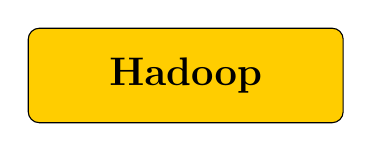
\begin{tikzpicture}[scale=0.8]
        \node[draw, rounded corners, fill=hadoopYellow, minimum width=4cm, minimum height=1.2cm, font=\Large\bfseries] {Hadoop};
      \end{tikzpicture}

      \vspace{1em}
      \small
      \begin{tabular}{ll}
        \faIcon{calendar} & 2006 -- present \\
        \faIcon{code-branch} & Version 3.x \\
        \faIcon{balance-scale} & Apache 2.0 License \\
        \faIcon{java} & Written in Java \\
      \end{tabular}
    \end{column}
  \end{columns}
\end{frame}

\begin{frame}{Why Hadoop?}
  \begin{alertblock}{The Problem}
    Data is growing exponentially: logs, IoT sensors, social media, transactions\ldots
    \\A single server can no longer store or process everything.
  \end{alertblock}

  \vspace{0.5em}

  \begin{exampleblock}{The Hadoop Solution}
    \begin{itemize}
      \item \textbf{Scale-out}: add more machines rather than buying a bigger one
      \item \textbf{Fault tolerance}: data is automatically replicated
      \item \textbf{Low cost}: runs on commodity hardware
      \item \textbf{Data locality}: computation moves to the data (not the other way around)
    \end{itemize}
  \end{exampleblock}
\end{frame}

\begin{frame}{The 3 Pillars of Hadoop}
  \centering
  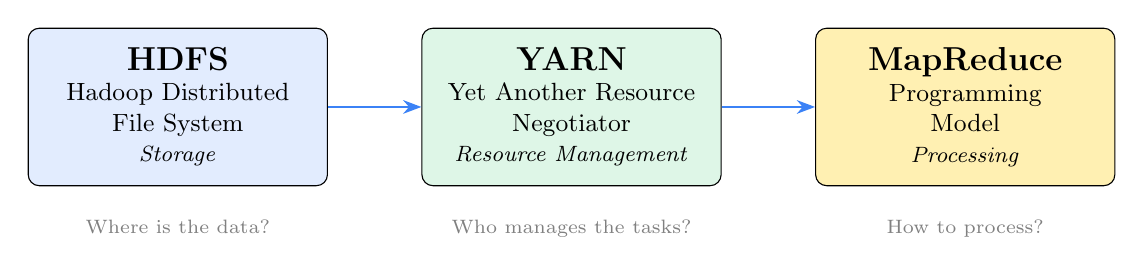
\begin{tikzpicture}[
    pillar/.style={draw, rounded corners, minimum width=3.8cm, minimum height=2cm,
                   align=center, font=\small},
    arr/.style={-{Stealth}, thick, hadoopBlue}
  ]
    \node[pillar, fill=hadoopBlue!15] (hdfs) at (0,0)
      {\textbf{\large HDFS}\\ Hadoop Distributed\\File System\\ \footnotesize\textit{Storage}};
    \node[pillar, fill=hadoopGreen!15] (yarn) at (5,0)
      {\textbf{\large YARN}\\ Yet Another Resource\\Negotiator\\ \footnotesize\textit{Resource Management}};
    \node[pillar, fill=hadoopYellow!30] (mr) at (10,0)
      {\textbf{\large MapReduce}\\ Programming\\Model\\ \footnotesize\textit{Processing}};

    \draw[arr] (hdfs) -- (yarn);
    \draw[arr] (yarn) -- (mr);

    \node[below=0.3cm of hdfs, font=\scriptsize\color{gray}] {Where is the data?};
    \node[below=0.3cm of yarn, font=\scriptsize\color{gray}] {Who manages the tasks?};
    \node[below=0.3cm of mr, font=\scriptsize\color{gray}] {How to process?};
  \end{tikzpicture}
\end{frame}

% ═════════════════════════════════════════════════════════════════════════════
\section{HDFS Architecture}
% ═════════════════════════════════════════════════════════════════════════════

\begin{frame}{HDFS -- Core Principles}
  \begin{columns}[T]
    \begin{column}{0.5\textwidth}
      \textbf{HDFS} = Hadoop Distributed File System.

      \vspace{0.5em}
      \begin{itemize}
        \item Files are split into \textbf{blocks} (128 MB by default)
        \item Each block is \textbf{replicated 3 times} across different machines
        \item Optimized for \textbf{sequential reads} of large files
        \item \textbf{Write-once, read-many} model
      \end{itemize}
    \end{column}
    \begin{column}{0.48\textwidth}
      \centering
      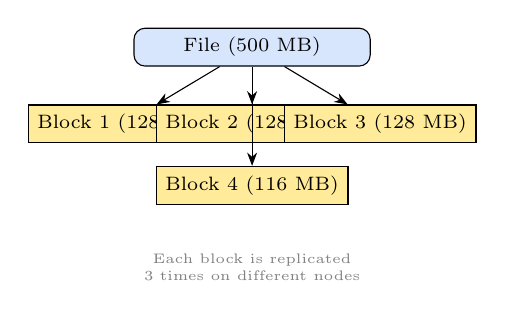
\begin{tikzpicture}[scale=0.65, every node/.style={font=\scriptsize}]
        \node[draw, fill=hadoopBlue!20, minimum width=3cm, rounded corners] (file) at (0,3) {File (500 MB)};

        \node[draw, fill=hadoopYellow!40, minimum width=1.8cm] (b1) at (-2.5,1.5) {Block 1 (128 MB)};
        \node[draw, fill=hadoopYellow!40, minimum width=1.8cm] (b2) at (0,1.5) {Block 2 (128 MB)};
        \node[draw, fill=hadoopYellow!40, minimum width=1.8cm] (b3) at (2.5,1.5) {Block 3 (128 MB)};
        \node[draw, fill=hadoopYellow!40, minimum width=1.8cm] (b4) at (0,0.3) {Block 4 (116 MB)};

        \draw[-{Stealth}] (file) -- (b1);
        \draw[-{Stealth}] (file) -- (b2);
        \draw[-{Stealth}] (file) -- (b3);
        \draw[-{Stealth}] (file) -- (b4);

        \node[below=0.5cm of b4, font=\tiny\color{gray}, align=center] {Each block is replicated\\3 times on different nodes};
      \end{tikzpicture}
    \end{column}
  \end{columns}
\end{frame}

\begin{frame}{HDFS -- NameNode / DataNode Architecture}
  \centering
  \begin{tikzpicture}[
    node distance=1.2cm and 1.5cm,
    box/.style={draw, rounded corners, minimum width=2.8cm, minimum height=1cm, align=center, font=\small},
    arr/.style={-{Stealth}, thick}
  ]
    % Client
    \node[box, fill=gray!15] (client) at (0, 3) {\faIcon{laptop} \textbf{Client}};

    % NameNode
    \node[box, fill=hadoopBlue!20] (nn) at (0, 1)
      {\faIcon{brain} \textbf{NameNode}\\\scriptsize Metadata};

    % DataNodes
    \node[box, fill=hadoopGreen!15] (dn1) at (-4, -1.5)
      {\faIcon{database} \textbf{DataNode 1}\\\scriptsize Blocks A, C};
    \node[box, fill=hadoopGreen!15] (dn2) at (0, -1.5)
      {\faIcon{database} \textbf{DataNode 2}\\\scriptsize Blocks A, B};
    \node[box, fill=hadoopGreen!15] (dn3) at (4, -1.5)
      {\faIcon{database} \textbf{DataNode 3}\\\scriptsize Blocks B, C};

    % Arrows
    \draw[arr, hadoopBlue] (client) -- node[right, font=\scriptsize] {1. Where is my file?} (nn);
    \draw[arr, hadoopBlue, dashed] (nn) -- node[right, font=\scriptsize] {2. Blocks on DN1, DN2, DN3} (client);
    \draw[arr, hadoopGreen!70!black] (client.west) -| node[above left, font=\scriptsize, pos=0.3] {3. Direct read} (dn1.north);

    % Heartbeats
    \draw[arr, gray, dotted] (dn1.north) -- node[left, font=\tiny, pos=0.3] {heartbeat} (nn.south west);
    \draw[arr, gray, dotted] (dn2.north) -- (nn.south);
    \draw[arr, gray, dotted] (dn3.north) -- node[right, font=\tiny, pos=0.3] {heartbeat} (nn.south east);
  \end{tikzpicture}
\end{frame}

\begin{frame}{HDFS Roles}
  \begin{table}
    \centering
    \begin{tabular}{lp{9cm}}
      \toprule
      \textbf{Component} & \textbf{Role} \\
      \midrule
      \textbf{NameNode} & Master server. Stores \textbf{metadata}: file tree, block locations, permissions. Does \textbf{not store any actual data}. \\
      \addlinespace
      \textbf{DataNode} & Worker server. Stores \textbf{data blocks} on local disk. Sends a \textit{heartbeat} to the NameNode every 3 seconds. \\
      \addlinespace
      \textbf{Client} & Reads/writes files via the NameNode (metadata) then communicates directly with DataNodes (data). \\
      \bottomrule
    \end{tabular}
  \end{table}
\end{frame}

% ═════════════════════════════════════════════════════════════════════════════
\section{YARN Architecture}
% ═════════════════════════════════════════════════════════════════════════════

\begin{frame}{YARN -- Resource Management}
  \centering
  \begin{tikzpicture}[
    node distance=1cm and 2cm,
    box/.style={draw, rounded corners, minimum width=3cm, minimum height=0.9cm, align=center, font=\small},
    arr/.style={-{Stealth}, thick}
  ]
    \node[box, fill=hadoopBlue!20] (rm) at (0, 2.5)
      {\faIcon{server} \textbf{ResourceManager}\\\scriptsize Global scheduler};

    \node[box, fill=hadoopGreen!15] (nm1) at (-4, 0)
      {\faIcon{microchip} \textbf{NodeManager 1}\\\scriptsize CPU + RAM};
    \node[box, fill=hadoopGreen!15] (nm2) at (0, 0)
      {\faIcon{microchip} \textbf{NodeManager 2}\\\scriptsize CPU + RAM};
    \node[box, fill=hadoopGreen!15] (nm3) at (4, 0)
      {\faIcon{microchip} \textbf{NodeManager 3}\\\scriptsize CPU + RAM};

    \node[box, fill=hadoopYellow!30] (am) at (0, -2)
      {\faIcon{tasks} \textbf{ApplicationMaster}\\\scriptsize Manages 1 job};

    \draw[arr] (rm) -- (nm1);
    \draw[arr] (rm) -- (nm2);
    \draw[arr] (rm) -- (nm3);
    \draw[arr, dashed, hadoopBlue] (am) -- node[right, font=\scriptsize] {requests containers} (rm);
    \draw[arr, hadoopGreen!70!black] (am) -- node[left, font=\scriptsize] {launches tasks} (nm1);
  \end{tikzpicture}

  \vspace{0.5em}
  \small
  \textbf{ResourceManager}: allocates cluster resources globally.\\
  \textbf{NodeManager}: manages resources on a single node.\\
  \textbf{ApplicationMaster}: coordinates the execution of one job.
\end{frame}

% ═════════════════════════════════════════════════════════════════════════════
\section{The MapReduce Model}
% ═════════════════════════════════════════════════════════════════════════════

\begin{frame}{MapReduce -- Overview}
  \centering
  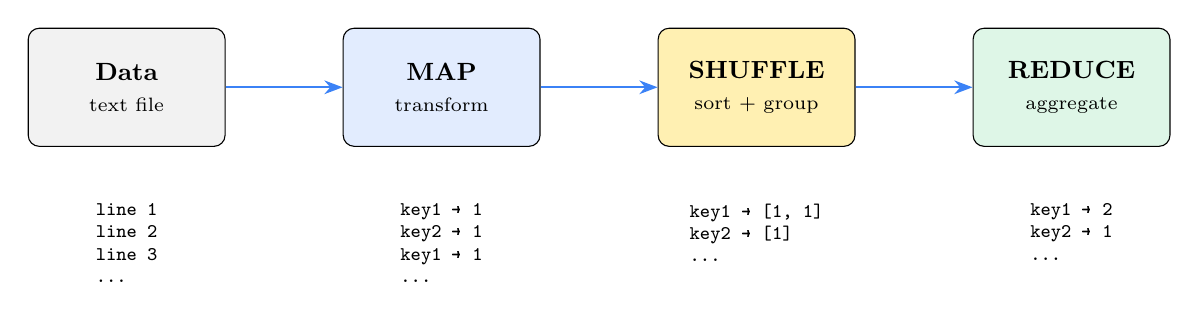
\begin{tikzpicture}[
    phase/.style={draw, rounded corners, minimum width=2.5cm, minimum height=1.5cm,
                  align=center, font=\small},
    data/.style={font=\scriptsize\ttfamily, align=left},
    arr/.style={-{Stealth}, thick, hadoopBlue}
  ]
    % Input
    \node[phase, fill=gray!10] (input) at (0, 0) {\textbf{Data}\\\scriptsize text file};

    % Map
    \node[phase, fill=hadoopBlue!15] (map) at (4, 0) {\textbf{MAP}\\\scriptsize transform};

    % Shuffle
    \node[phase, fill=hadoopYellow!30] (shuffle) at (8, 0) {\textbf{SHUFFLE}\\\scriptsize sort + group};

    % Reduce
    \node[phase, fill=hadoopGreen!15] (reduce) at (12, 0) {\textbf{REDUCE}\\\scriptsize aggregate};

    \draw[arr] (input) -- (map);
    \draw[arr] (map) -- (shuffle);
    \draw[arr] (shuffle) -- (reduce);

    % Annotations
    \node[data, below=0.6cm of input] {line 1\\line 2\\line 3\\...};
    \node[data, below=0.6cm of map] {key1 → 1\\key2 → 1\\key1 → 1\\...};
    \node[data, below=0.6cm of shuffle] {key1 → [1, 1]\\key2 → [1]\\...};
    \node[data, below=0.6cm of reduce] {key1 → 2\\key2 → 1\\...};
  \end{tikzpicture}
\end{frame}

\begin{frame}{MapReduce -- The 3 Phases in Detail}
  \begin{columns}[T]
    \begin{column}{0.32\textwidth}
      \begin{block}{\faIcon{expand-arrows-alt} MAP Phase}
        \begin{itemize}
          \item Reads data \textbf{line by line}
          \item Emits \texttt{key → value} pairs
          \item Runs in \textbf{parallel} on each node
          \item No communication between mappers
        \end{itemize}
      \end{block}
    \end{column}
    \begin{column}{0.32\textwidth}
      \begin{block}{\faIcon{sort-amount-down} SHUFFLE Phase}
        \begin{itemize}
          \item \textbf{Automatic} (handled by Hadoop)
          \item Sorts pairs by key
          \item Groups values by key
          \item Transfers data between nodes
        \end{itemize}
      \end{block}
    \end{column}
    \begin{column}{0.32\textwidth}
      \begin{block}{\faIcon{compress-arrows-alt} REDUCE Phase}
        \begin{itemize}
          \item Receives \texttt{key → [v1, v2, ...]}
          \item \textbf{Aggregates} values (sum, max, avg\ldots)
          \item Writes final result to HDFS
        \end{itemize}
      \end{block}
    \end{column}
  \end{columns}
\end{frame}

% ═════════════════════════════════════════════════════════════════════════════
\section{Docker Cluster Architecture}
% ═════════════════════════════════════════════════════════════════════════════

\begin{frame}{Our Cluster -- docker-compose}
  \centering
  \begin{tikzpicture}[
    cont/.style={draw, rounded corners, minimum width=3cm, minimum height=1.3cm,
                 align=center, font=\small},
    arr/.style={-{Stealth}, thick, gray}
  ]
    \node[cont, fill=hadoopBlue!15] (nn) at (0, 2)
      {\faIcon{brain} \textbf{namenode}\\\scriptsize Port 9870 (Web UI)\\\scriptsize Port 8020 (IPC)};
    \node[cont, fill=hadoopGreen!15] (dn) at (6, 2)
      {\faIcon{database} \textbf{datanode}\\\scriptsize Block storage};
    \node[cont, fill=hadoopYellow!30] (rm) at (0, -0.5)
      {\faIcon{server} \textbf{resourcemanager}\\\scriptsize Port 8088 (Web UI)};
    \node[cont, fill=hadoopRed!10] (nm) at (6, -0.5)
      {\faIcon{microchip} \textbf{nodemanager}\\\scriptsize Task execution};

    \draw[arr] (dn) -- node[above, font=\scriptsize] {hdfs://namenode:8020} (nn);
    \draw[arr] (nm) -- node[above, font=\scriptsize] {YARN} (rm);
    \draw[arr, dashed] (rm) -- node[left, font=\scriptsize] {depends on} (nn);
    \draw[arr, dashed] (nm) -- node[right, font=\scriptsize] {depends on} (rm);

    % Docker network
    \node[draw, dashed, gray, rounded corners, fit=(nn)(dn)(rm)(nm),
          inner sep=0.5cm, label={[font=\scriptsize\color{gray}]below:Docker network: hadoop\_default}] {};
  \end{tikzpicture}
\end{frame}

\begin{frame}[fragile]{docker-compose.yml}
  \begin{lstlisting}[language=bash, basicstyle=\ttfamily\tiny]
services:
  namenode:
    image: bde2020/hadoop-namenode:2.0.0-hadoop3.2.1-java8
    environment:
      - CLUSTER_NAME=test
      - CORE_CONF_fs_defaultFS=hdfs://namenode:8020
    ports:
      - "9870:9870"       # HDFS Web UI

  datanode:
    image: bde2020/hadoop-datanode:2.0.0-hadoop3.2.1-java8
    environment:
      - CORE_CONF_fs_defaultFS=hdfs://namenode:8020

  resourcemanager:
    image: bde2020/hadoop-resourcemanager:2.0.0-hadoop3.2.1-java8
    ports:
      - "8088:8088"       # YARN Web UI

  nodemanager:
    image: bde2020/hadoop-nodemanager:2.0.0-hadoop3.2.1-java8
  \end{lstlisting}

  \vspace{0.3em}
  \small
  \faIcon{terminal} Start: \texttt{docker compose up -d} \quad|\quad
  Stop: \texttt{docker compose down}
\end{frame}

% ═════════════════════════════════════════════════════════════════════════════
\section{Practical Case: Web Log Analysis}
% ═════════════════════════════════════════════════════════════════════════════

\begin{frame}{Practical Case -- Objective}
  \begin{block}{Scenario}
    A web server generates thousands of access log lines.\\
    We want to analyze these logs to extract meaningful statistics.
  \end{block}

  \vspace{0.5em}

  \textbf{Questions to answer:}
  \begin{enumerate}
    \item How many requests per \textbf{HTTP status code}? (200, 404, 500\ldots)
    \item Which are the \textbf{most visited pages}?
    \item What is the distribution by \textbf{HTTP method}? (GET, POST\ldots)
    \item How does \textbf{traffic vary by hour}?
  \end{enumerate}

  \vspace{0.5em}

  \begin{exampleblock}{Tools used}
    \textbf{HDFS} to store the logs \quad + \quad \textbf{MapReduce} (Hadoop Streaming + awk) to analyze them
  \end{exampleblock}
\end{frame}

\begin{frame}[fragile]{Data Format}
  Each log line follows the \textbf{Apache Combined Log} format:

  \vspace{0.3em}
  \begin{lstlisting}[basicstyle=\ttfamily\tiny]
192.168.1.10 - - [25/Mar/2026:10:00:01] "GET /index.html HTTP/1.1" 200 1024
192.168.1.12 - - [25/Mar/2026:10:00:03] "GET /missing.html HTTP/1.1" 404 512
192.168.1.15 - - [25/Mar/2026:10:00:07] "GET /api/data HTTP/1.1" 500 64
  \end{lstlisting}

  \vspace{0.5em}
  \textbf{Field breakdown} (space-separated):

  \vspace{0.3em}
  \centering
  \begin{tabular}{clll}
    \toprule
    \textbf{Field} & \textbf{Name} & \textbf{Example} & \textbf{Usage} \\
    \midrule
    \texttt{\$1} & IP address & 192.168.1.10 & -- \\
    \texttt{\$4} & Date/Time & [25/Mar/2026:10:00:01] & Hourly traffic \\
    \texttt{\$5} & Method & "GET & GET/POST distribution \\
    \texttt{\$6} & Page & /index.html & Most visited pages \\
    \texttt{\$8} & HTTP code & 200 & Response codes \\
    \texttt{\$9} & Size & 1024 & Transferred volume \\
    \bottomrule
  \end{tabular}
\end{frame}

\begin{frame}{Mechanism -- Processing Pipeline}
  \centering
  \begin{tikzpicture}[
    step/.style={draw, rounded corners, minimum width=3cm, minimum height=1cm,
                 align=center, font=\small},
    arr/.style={-{Stealth}, very thick, hadoopBlue}
  ]
    \node[step, fill=gray!10] (gen) at (0, 3) {\faIcon{file-alt} \textbf{Generate logs}\\\scriptsize 10,000 lines};
    \node[step, fill=hadoopBlue!15] (hdfs) at (0, 1.2) {\faIcon{upload} \textbf{Load into HDFS}\\\scriptsize \texttt{hdfs dfs -put}};
    \node[step, fill=hadoopYellow!30] (map) at (-4, -0.6) {\faIcon{expand-arrows-alt} \textbf{MAP}\\\scriptsize Extract fields};
    \node[step, fill=orange!15] (shuf) at (0, -0.6) {\faIcon{sort-amount-down} \textbf{SHUFFLE}\\\scriptsize Sort by key};
    \node[step, fill=hadoopGreen!15] (red) at (4, -0.6) {\faIcon{compress-arrows-alt} \textbf{REDUCE}\\\scriptsize Aggregate};
    \node[step, fill=hadoopBlue!10] (out) at (0, -2.5) {\faIcon{chart-bar} \textbf{Result}\\\scriptsize HTML Dashboard};

    \draw[arr] (gen) -- (hdfs);
    \draw[arr] (hdfs.south) -- ++(0,-0.3) -| (map.north);
    \draw[arr] (map) -- (shuf);
    \draw[arr] (shuf) -- (red);
    \draw[arr] (red.south) -- ++(0,-0.3) -| (out.north);
  \end{tikzpicture}
\end{frame}

\begin{frame}[fragile]{The Mapper (awk)}
  The mapper reads each line and emits \texttt{key<TAB>value} pairs:

  \begin{lstlisting}[language=awk]
BEGIN { OFS = "\t" }
{
    code = $8             # HTTP code (200, 404, 500...)
    if (code ~ /^[0-9]+$/) {
        print code, 1     # Emits: 200<TAB>1
    }
}
  \end{lstlisting}

  \vspace{0.3em}
  \textbf{Input} (1 log line):
  \begin{lstlisting}[basicstyle=\ttfamily\tiny]
192.168.1.10 - - [25/Mar/2026:10:00:01] "GET /index.html HTTP/1.1" 200 1024
  \end{lstlisting}

  \textbf{Output}:
  \begin{lstlisting}[basicstyle=\ttfamily\small]
200     1
  \end{lstlisting}
\end{frame}

\begin{frame}[fragile]{The Reducer (awk)}
  The reducer receives pairs \textbf{sorted by key} and sums the counters:

  \begin{lstlisting}[language=awk]
BEGIN { FS = "\t"; OFS = "\t" }
{
    if ($1 == prev) {
        count += $2       # Same key: accumulate
    } else {
        if (prev != "") print prev, count
        prev = $1         # New key
        count = $2
    }
}
END { if (prev != "") print prev, count }
  \end{lstlisting}

  \vspace{0.3em}
  \textbf{Input} (sorted by Hadoop):
  \begin{lstlisting}[basicstyle=\ttfamily\small]
200     1
200     1
200     1
404     1
404     1
  \end{lstlisting}

  \textbf{Output}:
  \begin{lstlisting}[basicstyle=\ttfamily\small]
200     3
404     2
  \end{lstlisting}
\end{frame}

\begin{frame}[fragile]{Running the Job}
  \begin{lstlisting}[language=bash, basicstyle=\ttfamily\scriptsize]
hadoop jar hadoop-streaming-3.2.1.jar \
    -D stream.num.map.output.key.fields=2 \
    -files /tmp/mapper.awk,/tmp/reducer.awk \
    -mapper  "awk -f /tmp/mapper.awk" \
    -reducer "awk -f /tmp/reducer.awk" \
    -input  /user/root/input/access.log \
    -output /user/root/output/results
  \end{lstlisting}

  \vspace{0.5em}
  \textbf{What Hadoop does:}
  \begin{enumerate}
    \item Splits the input file into \textbf{input splits}
    \item Runs the \textbf{mapper} on each split (in parallel across DataNodes)
    \item \textbf{Sorts and groups} key-value pairs (shuffle)
    \item Runs the \textbf{reducer} to aggregate results
    \item Writes output to HDFS (\texttt{part-00000})
  \end{enumerate}
\end{frame}

% ═════════════════════════════════════════════════════════════════════════════
\section{Expected Results}
% ═════════════════════════════════════════════════════════════════════════════

\begin{frame}{Results -- HTTP Status Codes}
  \begin{columns}[T]
    \begin{column}{0.45\textwidth}
      \begin{table}
        \centering
        \begin{tabular}{cr}
          \toprule
          \textbf{Code} & \textbf{Requests} \\
          \midrule
          \textcolor{hadoopGreen}{200 OK} & 5,846 \\
          \textcolor{hadoopBlue}{301 Redirect} & 812 \\
          \textcolor{orange}{403 Forbidden} & 841 \\
          \textcolor{hadoopYellow!80!black}{404 Not Found} & 809 \\
          \textcolor{hadoopRed}{500 Server Error} & 835 \\
          \textcolor{hadoopRed!70}{502 Bad Gateway} & 857 \\
          \midrule
          \textbf{Total} & \textbf{10,000} \\
          \bottomrule
        \end{tabular}
      \end{table}
    \end{column}
    \begin{column}{0.5\textwidth}
      \textbf{Interpretation:}
      \begin{itemize}
        \item \textasciitilde58\% successful (200)
        \item \textasciitilde17\% server errors (5xx)
        \item \textasciitilde8\% not found (404)
        \item \textasciitilde8\% access denied (403)
      \end{itemize}

      \vspace{0.5em}
      \begin{alertblock}{\scriptsize Action Item}
        500/502 error rates are high $\rightarrow$ investigate endpoints \texttt{/api/crash} and \texttt{/api/timeout}.
      \end{alertblock}
    \end{column}
  \end{columns}
\end{frame}

\begin{frame}{Results -- Pages and Methods}
  \begin{columns}[T]
    \begin{column}{0.48\textwidth}
      \textbf{Top 5 most visited pages:}
      \vspace{0.3em}
      \begin{table}
        \centering
        \begin{tabular}{lr}
          \toprule
          \textbf{Page} & \textbf{Hits} \\
          \midrule
          /login & 439 \\
          /deprecated & 431 \\
          /search & 423 \\
          /api/timeout & 418 \\
          /blog/post-2 & 416 \\
          \bottomrule
        \end{tabular}
      \end{table}
    \end{column}
    \begin{column}{0.48\textwidth}
      \textbf{HTTP method distribution:}
      \vspace{0.3em}
      \begin{table}
        \centering
        \begin{tabular}{lr}
          \toprule
          \textbf{Method} & \textbf{Requests} \\
          \midrule
          GET & 5,757 (57.6\%) \\
          POST & 1,438 (14.4\%) \\
          PUT & 1,412 (14.1\%) \\
          DELETE & 1,393 (13.9\%) \\
          \bottomrule
        \end{tabular}
      \end{table}

      \vspace{0.3em}
      \small
      \faIcon{info-circle} Traffic is mostly GET (read-heavy).
    \end{column}
  \end{columns}
\end{frame}

\begin{frame}{Results -- Hourly Traffic}
  \centering
  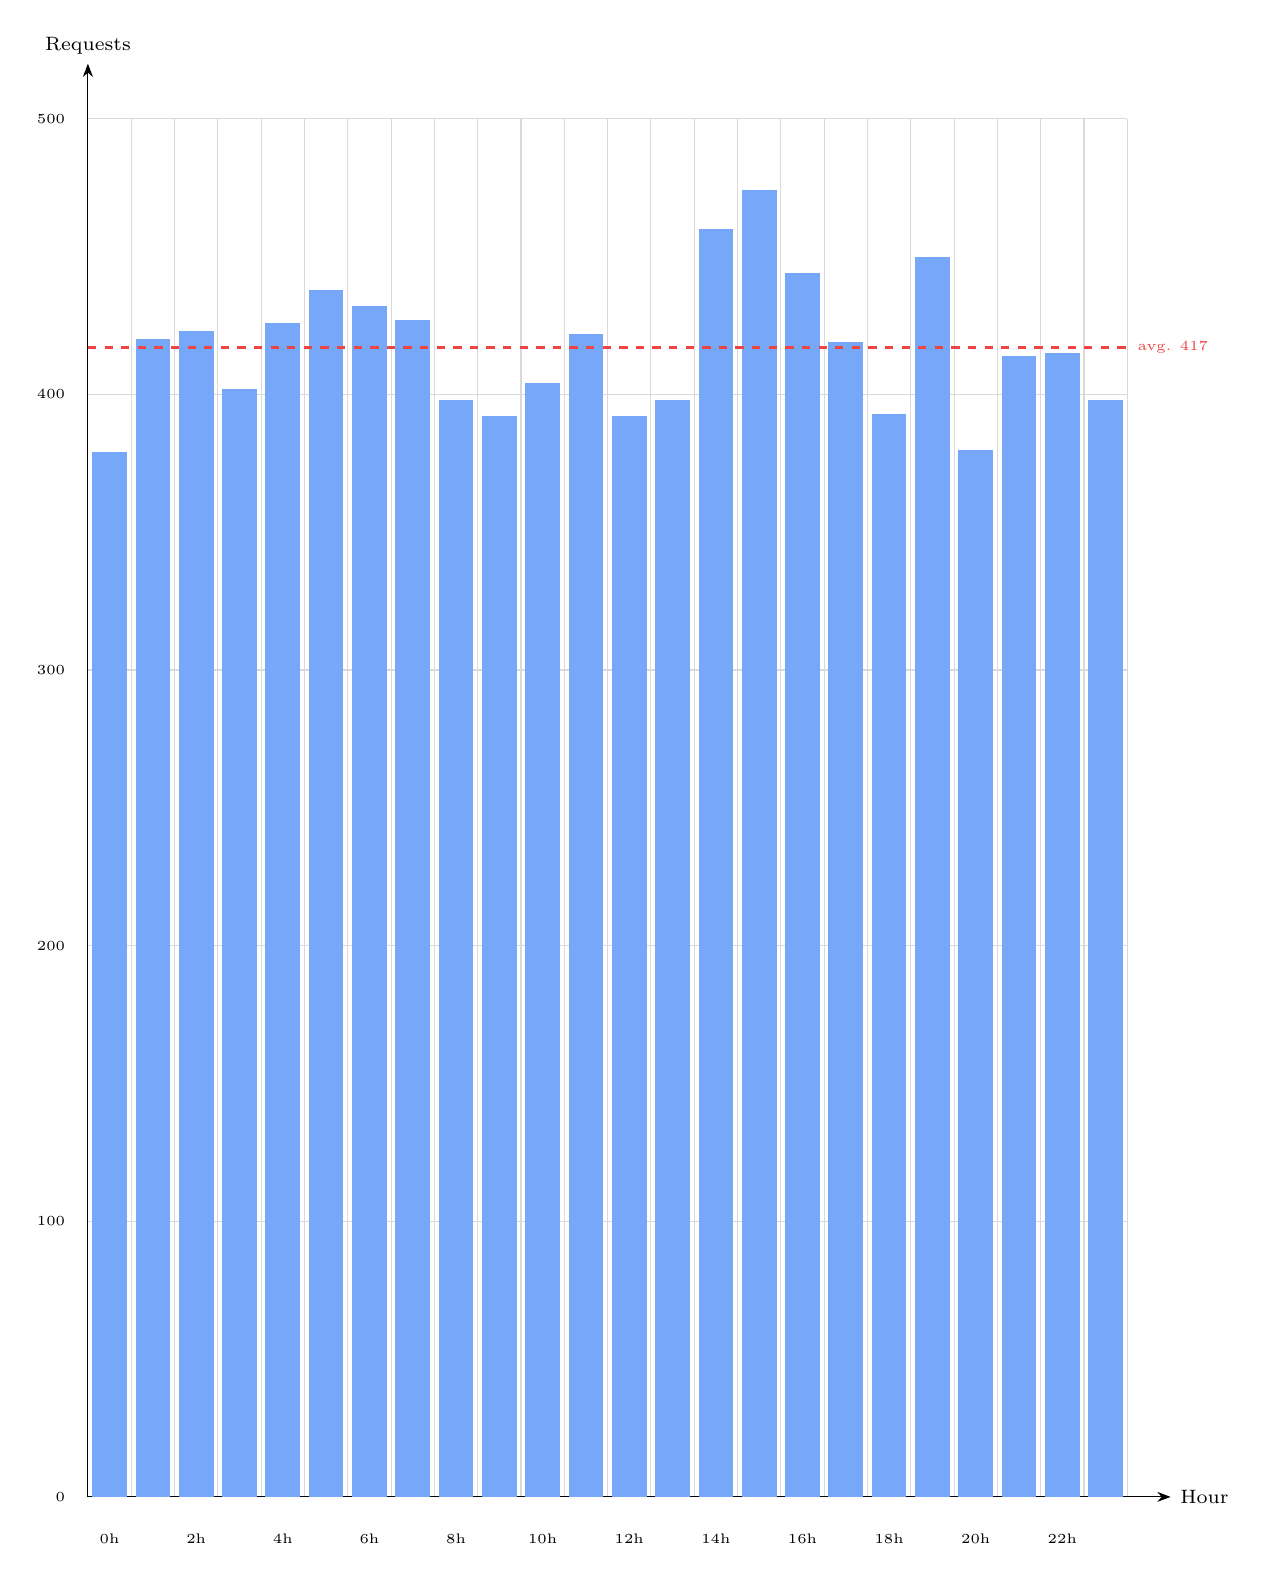
\begin{tikzpicture}[xscale=0.55, yscale=0.035]
    \draw[gray!30, thin] (0,0) grid[xstep=1, ystep=100] (24, 500);
    \draw[-{Stealth}] (0,0) -- (25,0) node[right, font=\scriptsize] {Hour};
    \draw[-{Stealth}] (0,0) -- (0,520) node[above, font=\scriptsize] {Requests};

    % Y axis labels
    \foreach \y in {0, 100, 200, 300, 400, 500} {
      \draw (-0.3, \y) node[left, font=\tiny] {\y};
    }
    % X axis labels
    \foreach \x in {0,2,...,22} {
      \draw (\x+0.5, -15) node[font=\tiny] {\x h};
    }

    % Bars
    \foreach \x/\val in {
      0/379, 1/420, 2/423, 3/402, 4/426, 5/438,
      6/432, 7/427, 8/398, 9/392, 10/404, 11/422,
      12/392, 13/398, 14/460, 15/474, 16/444, 17/419,
      18/393, 19/450, 20/380, 21/414, 22/415, 23/398} {
      \fill[hadoopBlue!70] (\x+0.1, 0) rectangle (\x+0.9, \val);
    }

    % Average line
    \draw[hadoopRed, thick, dashed] (0, 417) -- (24, 417) node[right, font=\tiny] {avg. 417};
  \end{tikzpicture}

  \vspace{0.5em}
  \small
  Traffic spread over 24h. Peak at \textbf{3 PM} (474 req.) -- lowest at \textbf{midnight} (379 req.).
\end{frame}

% ═════════════════════════════════════════════════════════════════════════════
\section{Dashboard \& Monitoring}
% ═════════════════════════════════════════════════════════════════════════════

\begin{frame}{Monitoring Interfaces}
  \begin{columns}[T]
    \begin{column}{0.48\textwidth}
      \begin{block}{\faIcon{hdd} HDFS -- \texttt{localhost:9870}}
        \begin{itemize}
          \item Cluster status
          \item Capacity and usage
          \item Active datanodes
          \item HDFS file browser
        \end{itemize}
      \end{block}
    \end{column}
    \begin{column}{0.48\textwidth}
      \begin{block}{\faIcon{tasks} YARN -- \texttt{localhost:8088}}
        \begin{itemize}
          \item Application list
          \item Job status (SUCCEEDED, FAILED)
          \item Number of mappers / reducers
          \item Execution time and logs
        \end{itemize}
      \end{block}
    \end{column}
  \end{columns}

  \vspace{1em}

  \begin{exampleblock}{\faIcon{chart-bar} Generated Dashboard -- \texttt{localhost:8888}}
    The \texttt{run-cas-pratique.sh} script automatically generates an interactive HTML dashboard
    with Chart.js graphs: doughnut (codes), bar (hours, pages), pie (methods).
  \end{exampleblock}
\end{frame}

% ═════════════════════════════════════════════════════════════════════════════
\section{Conclusion}
% ═════════════════════════════════════════════════════════════════════════════

\begin{frame}{Key Takeaways}
  \begin{columns}[T]
    \begin{column}{0.48\textwidth}
      \textbf{Hadoop enables:}
      \begin{itemize}
        \item Distributed storage of massive data (\textbf{HDFS})
        \item Parallel data processing (\textbf{MapReduce})
        \item Cluster resource management (\textbf{YARN})
        \item Automatic fault tolerance
      \end{itemize}
    \end{column}
    \begin{column}{0.48\textwidth}
      \textbf{In our practical case:}
      \begin{itemize}
        \item 10,000 logs analyzed in minutes
        \item 4 dimensions extracted (codes, pages, methods, hours)
        \item Reproducible pipeline: single script
        \item Results viewable in the browser
      \end{itemize}
    \end{column}
  \end{columns}

  \vspace{1em}
  \centering
  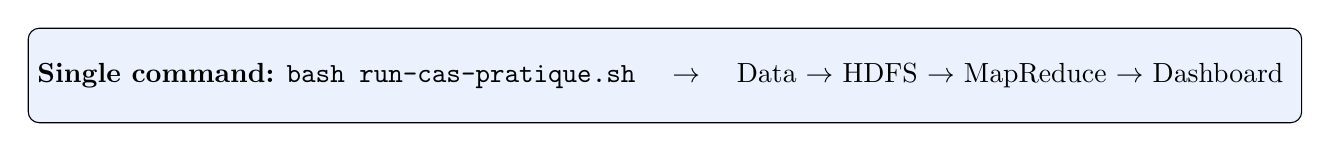
\begin{tikzpicture}
    \node[draw, rounded corners, fill=hadoopBlue!10, minimum width=12cm, minimum height=1.2cm, align=center] {
      \textbf{Single command:} \texttt{bash run-cas-pratique.sh}
      \quad $\rightarrow$ \quad Data $\rightarrow$ HDFS $\rightarrow$ MapReduce $\rightarrow$ Dashboard
    };
  \end{tikzpicture}
\end{frame}

\begin{frame}{}
  \centering
  \vspace{2cm}
  {\Huge\bfseries Thank you!}

  \vspace{1.5em}
  {\large Questions?}

  \vspace{2em}
  \small
  \begin{tabular}{cl}
    \faIcon{github} & \texttt{github.com/Achaire-Zogo/hadoop} \\
    \faIcon{globe} & Dashboard: \texttt{http://localhost:8888/dashboard.html} \\
    \faIcon{terminal} & \texttt{bash run-cas-pratique.sh} \\
  \end{tabular}
\end{frame}

\end{document}
